\documentclass[
	11pt
] {article}

\usepackage[
	a4paper,
	left=3cm,
	right=3cm,
	top=3cm,
	bottom=3cm,
	headheight=1cm
] {geometry} %for setting margin

\usepackage{fancyhdr} %for header and footers
\usepackage{parskip} %for leaving some space after paragraphs


% Math
\usepackage{mathtools} %helps to number equations
\usepackage{siunitx} % Units of measurement


% For graphs and advanced diagrams
\usepackage{tikz} %the drawing library
\usetikzlibrary{positioning} %some auxilary to the drawing library
\usetikzlibrary{math} %helps to define variables in the tikz

\usepackage{authblk} %authors and their affiliations

% Basic graphics
\usepackage{float} %to force the figure to be in a place among the text
\usepackage{graphicx} %for include graphics
\usepackage{caption} %better referencing to labels
\usepackage{subcaption}  %helps with multiple pictures in a figure


% Language and Font package: COMMENT THESE FOR ENGLISH ONLY
\usepackage[T2A]{fontenc} %[RUS] loads cyrillic characters
\usepackage[russian]{babel} %[RUS] changes date heading 'abstract' to Russian
\usepackage[utf8]{inputenc} %[RUS] to force utf-8 encoding

\usepackage{hyperref}
\usepackage{pythonhighlight}


%-----------------------------------------------------------------------

\renewcommand\thesubfigure{\asbuk{subfigure}} %[RUS] for renaming subfigures to russian
\sisetup{output-decimal-marker = {,}} %[RUS] changes all ordinary decimal separator to rassiky commas
\pagestyle{fancy}
\graphicspath{{figures/}}

\newcommand\authFirst{Лебедев Матвей}
\newcommand\authSecond{Шаббир Кафи}
\newcommand\titleLong{Проект по анализу данных на Python: Богатый домовладелец}
\newcommand\titleShort{Богатый домовладелец}

\author[1, a]{\authFirst{}}
\author[1, b]{\authSecond{}}


\affil[1]{Московский физико-технический институт, Долгопрудный, 141701}
\affil[a]{lebedev.ma@phystech.edu М02-301я}
\affil[b]{kafiulshabbir@phystech.edu M03-304б}

\title{\titleLong}
\fancyhead{}
\fancyhead[L]{\titleShort}
\fancyhead[R]{\authFirst{}, \authSecond{}}
\fancyhead[C]{\the\year}



\begin{document}
% \nocite{*}

\maketitle


\begin{abstract}
	В последние годы рынок краткосрочной аренды жилья через платформы, такие как Airbnb, существенно вырос. Тем не менее, существует ограниченное понимание того, какие факторы наиболее сильно влияют на цены листингов. Это знание может помочь как владельцам жилья, так и арендаторам лучше ориентироваться на рынке.
\end{abstract}

\tableofcontents
\section{Введение}

\subsection{Проблема}
	В последние годы рынок краткосрочной аренды жилья через платформы, такие как Airbnb, существенно вырос \cite{guttentag2019progress}. Тем не менее, существует ограниченное понимание того, какие факторы наиболее сильно влияют на цены листингов. Это знание может помочь как владельцам жилья, так и арендаторам лучше ориентироваться на рынке \cite{halket2020housing}.

\subsection{Актуальность}
	 Для владельцев жилья знание факторов, влияющих на цену, поможет оптимизировать свои предложения, а для арендаторов — выбрать наиболее выгодные варианты.

\subsection{Исследовательский вопрос}
	Какие факторы объясняют вариации цен на листинги Airbnb в Амстердаме в будние дни?

\subsection{Гипотезы}
	\begin{enumerate}
		\item Листинги, расположенные ближе к центру города, имеют более высокие цены.
		\item Листинги, предоставляемые суперхостами, имеют более высокие цены.
		\item Листинги с большим количеством спален имеют более высокие цены.
		\item Листинги с высоким рейтингом удовлетворенности гостей имеют более высокие цены.
		\item Листинги, предлагающие целый дом или квартиру, имеют более высокие цены по сравнению с отдельными комнатами.
		\item Листинги, расположенные ближе к популярным туристическим местам, имеют более высокие цены.
		\item Листинги, находящиеся в районах с высоким уровнем бизнеса (biz), имеют более высокие цены.
		\item Листинги с более высоким значением cleanliness\_rating имеют более высокую цену.
		\item Листинги, доступные для бронирования на несколько комнат (multi), имеют более высокие цены.
	\end{enumerate}

\section{Методология}

\subsection{Методы сбора данных}
	Данные собраны и предоставлены в виде CSV-файла. Источник данных - платформа Airbnb

\subsection{Описание данных}
	Данные содержат информацию о краткосрочной аренде жилья в Амстердаме в будние дни. Каждый объект недвижимости представлен множеством характеристик, включая тип комнаты, вместимость, оценки чистоты и удовлетворенности гостей, а также различные индексы привлекательности и доступности ресторанов. Данные могут использоваться для анализа факторов, влияющих на цены и популярность аренды, а также для оценки качества обслуживания.

	Файл: amsterdam\_weekends.csv \cite{kaggleAirbnbPrices}.

\subsection{Столбцы данных}
	\begin{enumerate}
		\item \textbf{Unnamed:} 0: Идентификатор записи (тип: числовой)
		\item \textbf{realSum:} Реальная сумма, стоимость проживания (тип: числовой)
		\item \textbf{room\_type:} Тип комнаты (категориальный)
		\item \textbf{room\_shared:} Комната общая (бинарный)
		\item \textbf{room\_private:} Комната частная (бинарный)
		\item \textbf{person\_capacity:} Вместимость комнаты (тип: числовой)
		\item \textbf{host\_is\_superhost:} Хост является супер-хостом (бинарный)
		\item \textbf{multi:} Количество объектов (тип: числовой)
		\item \textbf{biz:} Бизнес-категория (тип: числовой)
		\item \textbf{cleanliness\_rating:} Оценка чистоты (тип: числовой)
		\item \textbf{guest\_satisfaction\_overall:} Общая удовлетворенность гостей (тип: числовой)
		\item \textbf{bedrooms:} Количество спален (тип: числовой)
		\item \textbf{dist:} Расстояние до центра (тип: числовой)
		\item \textbf{metro\_dist:} Расстояние до метро (тип: числовой)
		\item \textbf{attr\_index:} Индекс привлекательности (тип: числовой)
		\item \textbf{attr\_index\_norm:} Нормированный индекс близости к туристическим местам (тип: числовой)
		\item \textbf{rest\_index:} Индекс ресторанов (тип: числовой)
		\item \textbf{rest\_index\_norm:} Нормированный индекс ресторанов (тип: числовой)
		\item \textbf{lng:} Долгота (тип: числовой)
		\item \textbf{lat:} Широта (тип: числовой)
	\end{enumerate}

\subsection{Аналитические методы}
	\begin{enumerate}
		\item Визуализация данных: Использование гистограмм, scatter plot, box plot и heatmap для анализа распределения данных и зависимостей между переменными.

		\item Описательная статистика: Средние значения, медианы, стандартные отклонения и другие описательные статистики для ключевых переменных \cite{mishra2019descriptive}.

		\item Корреляционный анализ: Определение корреляций между переменными с помощью коэффициента корреляции Пирсона \cite{cohen2009pearson}.

		\item T-тест: Сравнение средних значений между двумя группами \cite{kim2015t}.
	\end{enumerate}

\subsection{Настройка программы для считывания данных}
	Импорт библиотек

\begin{python}
import pandas as pd
import matplotlib.pyplot as plt
import seaborn as sns
from scipy.stats import ttest_ind
%matplotlib inline
\end{python}

	Считываем данные и предобрабатываем

\begin{python}
file_path = 'amsterdam_weekdays.csv'
df = pd.read_csv(file_path)
df.head()
\end{python}

	\begin{figure}[H]
		\centering
		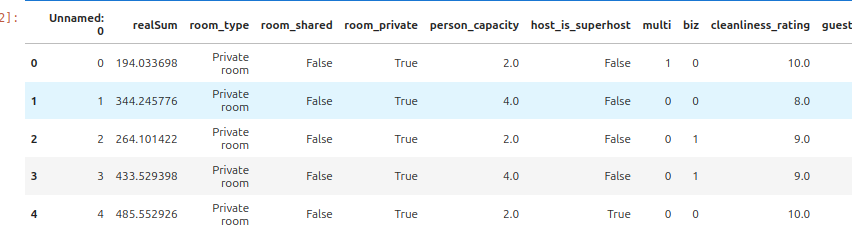
\includegraphics[width=1.0\textwidth]{fig-00}
		\caption{Как выглядят наши данные после импорта. А справа есть еще много столб.}
	\end{figure}

\section{Результаты}

\subsection{Корреляционная матрица}
\begin{python}
correlation_matrix = df[['realSum', 'dist', 'bedrooms', 'guest_satisfaction_overall', 'attr_index', 'multi', 'biz', 'cleanliness_rating']].corr()

plt.figure(figsize=(10, 8))
sns.heatmap(correlation_matrix, annot=True, cmap='coolwarm', fmt=".2f")
plt.title('Correlation Matri')
plt.show()
\end{python}

	\begin{figure}[H]
		\centering
		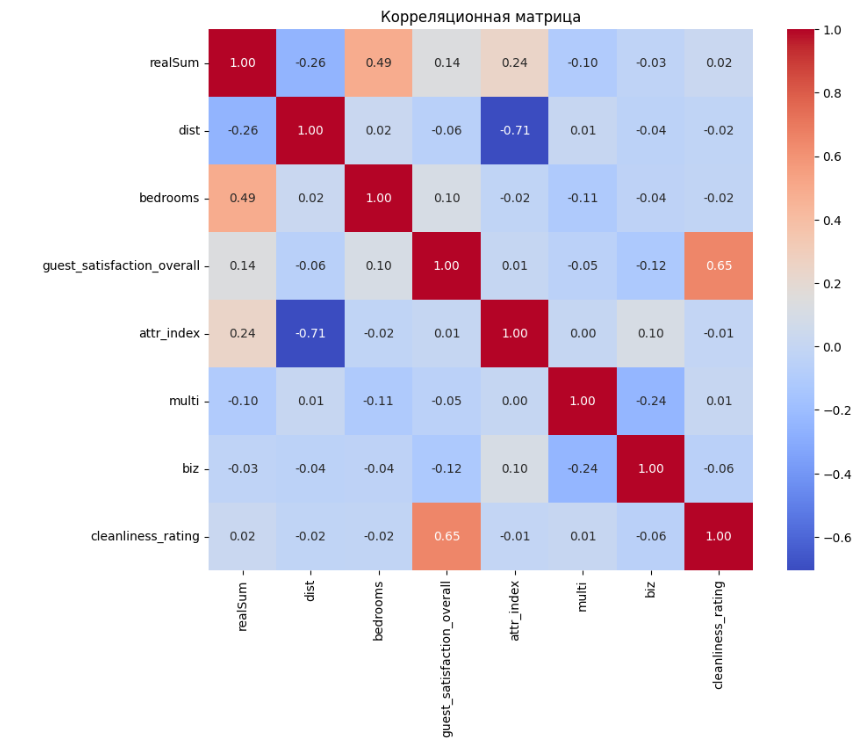
\includegraphics[width=1.0\textwidth]{fig-01}
		\caption{тепловая карта корреляций.}
	\end{figure}

\subsection{Цены в зависимости от расстояния до центра города}
\begin{python}
plt.figure(figsize=(10, 6))
sns.scatterplot(data=df, x='dist', y='realSum', hue='dist', palette='coolwarm')
plt.title('Prices depending on the distance to the city center')
plt.xlabel('Distance to the city center (dist)')
plt.ylabel('Price (realSum)')
plt.show()
\end{python}

	\begin{figure}[H]


		\centering
		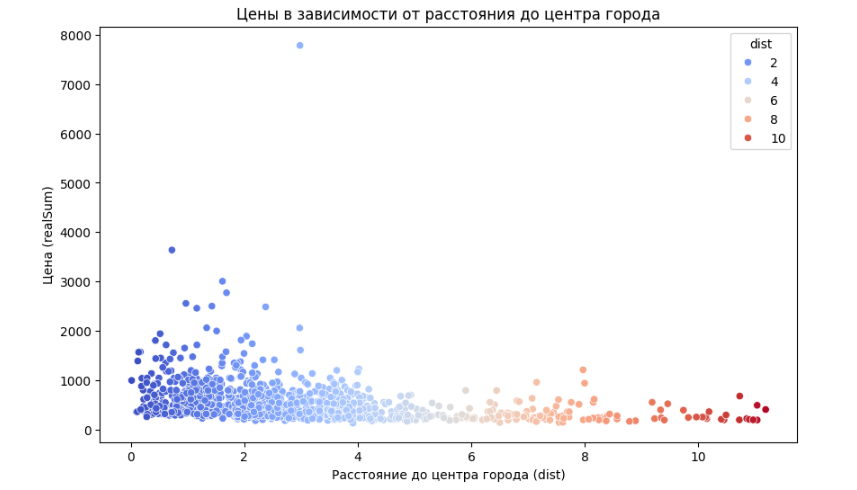
\includegraphics[width=1.0\textwidth]{fig-02}
		\caption{для наших гипотез, чтобы подкрепить наши выводы из кореляционного анализа и описательной статистики. Листинги, расположенные ближе к центру города, имеют более высокие цены.}
	\end{figure}

	Значение корреляции между переменными -0.26, что говорит об небольшой обратной связи - чем меньше расстояние до центра, тем выше цена, это и подтверждается по графику, потому что видим сильное скопление точек на высоких значениях цен у малого значения dist и наоборот малое значение цены у точек с максимальной dist. Гипотеза подтверждается.

\subsection{Цены в зависимости от того, является ли хозяин суперхостом}
\begin{python}
plt.figure(figsize=(10, 6))
sns.boxplot(data=df, x='host_is_superhost', y='realSum')
plt.title('Prices depending on whether the host is a superhost')
plt.xlabel('Superhost')
plt.ylabel('Price (realSum)')
plt.show()

# t-test
superhost_prices = df[df['host_is_superhost'] == True]['realSum']
non_superhost_prices = df[df['host_is_superhost'] == False]['realSum']
t_stat_superhost, p_val_superhost = ttest_ind(superhost_prices, non_superhost_prices)
t_stat_superhost, p_val_superhost

# (-2.0985191376128354, 0.03608667618036517)

\end{python}

	\begin{figure}[H]
		\centering
		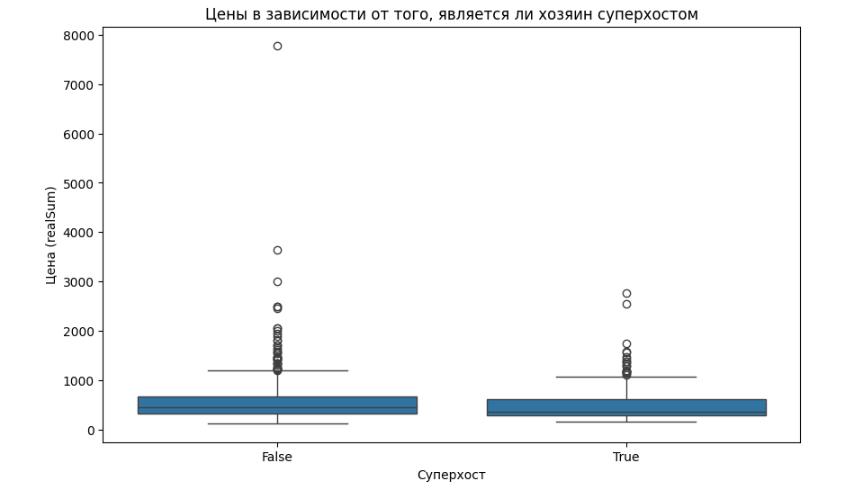
\includegraphics[width=1.0\textwidth]{fig-03}
		\caption{Листинги, предоставляемые суперхостами, имеют более высокие цены.}
	\end{figure}
	Построили диарамму с усами и видим, что медианное значение ниже у True, но слабо заметно на графике, поэтому мы дополнительно сделали t-test и увидели значимую разницу в ценах причем цена у True Ниже. Гипотеза отвергается.

\subsection{Цены в зависимости от количества спален}
\begin{python}
plt.figure(figsize=(10, 6))
sns.boxplot(data=df, x='bedrooms', y='realSum')
plt.title('Prices depending on the number of bedrooms')
plt.xlabel('Number of bedrooms (bedrooms)')
plt.ylabel('Price (realSum)')
plt.show()
\end{python}

	\begin{figure}[H]
		\centering
		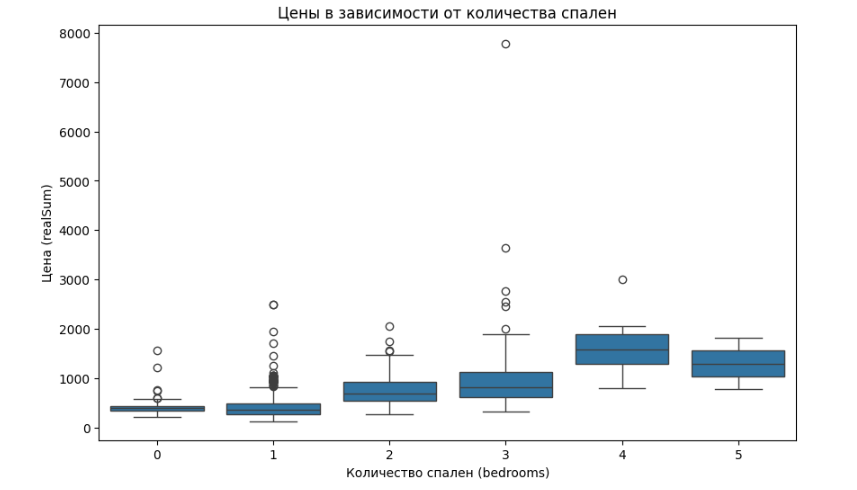
\includegraphics[width=1.0\textwidth]{fig-04}
		\caption{Листинги с большим количеством спален имеют более высокие цены.}
	\end{figure}

	Построили диарамму с усами и видим, что медианное значение растет до 4 спален, но потом становится ниже, но это некритично, также наличие корреляции между переменными 0.49, что говорит о наличии положительной связи между переменными.


\subsection{Цены в зависимости от рейтинга удовлетворенности гостей}
\begin{python}
plt.figure(figsize=(10, 6))
sns.scatterplot(data=df, x='guest_satisfaction_overall', y='realSum', hue='guest_satisfaction_overall', palette='viridis')
plt.title('Prices depending on guest satisfaction rating')
plt.xlabel('Guest Satisfaction rating (guest_satisfaction_overall)')
plt.ylabel('Price (realSum)')
plt.show()
\end{python}

	\begin{figure}[H]
		\centering
		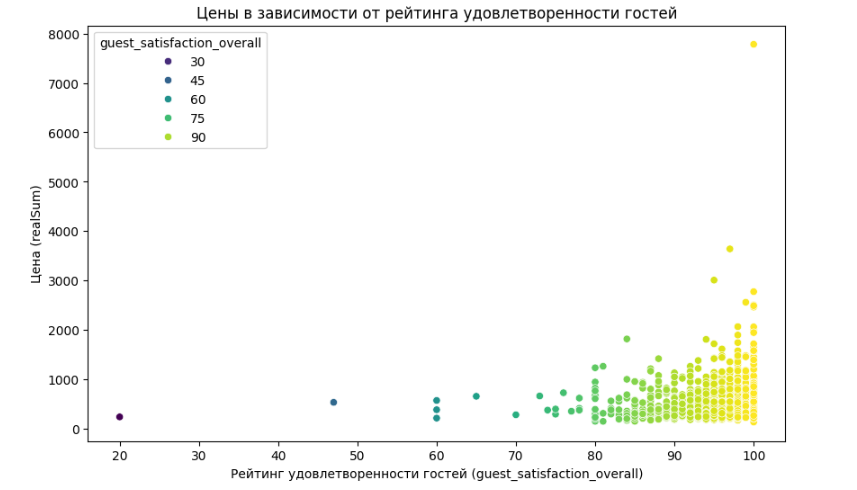
\includegraphics[width=1.0\textwidth]{fig-05}
		\caption{Листинги с высоким рейтингом удовлетворенности гостей имеют более высокие цены.}
	\end{figure}

	По точечной диаграмме мы видим положительный тренд и можем сказать, что рейтинг удовлетворенности гостей влияет на цену. Корреляция между переменными 0.14, что говорит о наличии малой положительной линейной зависимости


\subsection{Цены в зависимости от типа листинга}
\begin{python}
plt.figure(figsize=(10, 6))
sns.boxplot(data=df, x='room_type', y='realSum')
plt.title('Prices depending on the type of listing')
plt.xlabel('Listing type (room_type)')
plt.ylabel('Price (realSum)')
plt.show()

# t-test
entire_home_prices = df[df['room_type'] == 'Shared room']['realSum']
private_room_prices = df[df['room_type'] == 'Private room']['realSum']
t_stat_room_type, p_val_room_type = ttest_ind(entire_home_prices, private_room_prices)
t_stat_room_type, p_val_room_type

# (-1.1628609255034663, 0.24537858346227584)
\end{python}

	\begin{figure}[H]
		\centering
		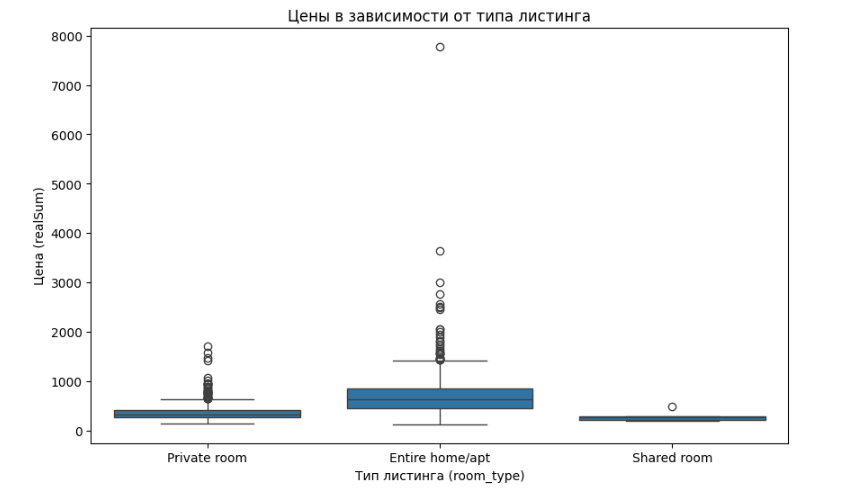
\includegraphics[width=1.0\textwidth]{fig-06}
		\caption{Листинги, предлагающие целый дом или квартиру, имеют более высокие цены по сравнению с отдельными комнатами.}
	\end{figure}

	По диаграмме с усами мы видим, что дом дороже квартиры и отдельных комнат, но проведенный t-test показывает, что нет статистической разницы между квартиры и отдельной комнаты, поэтому можем принять гипотезу частично и сказать, что дом - самый дорой тип листинга


\subsection{Цены в зависимости от близости к популярным туристическим местам}
\begin{python}
plt.figure(figsize=(10, 6))
sns.scatterplot(data=df, x='attr_index', y='realSum', hue='attr_index', palette='coolwarm')
plt.title('Prices depending on proximity to popular tourist spots')
plt.xlabel('Index of proximity to tourist places (attr_index)')
plt.ylabel('Price (realSum)')
plt.show()
\end{python}

	\begin{figure}[H]
		\centering
		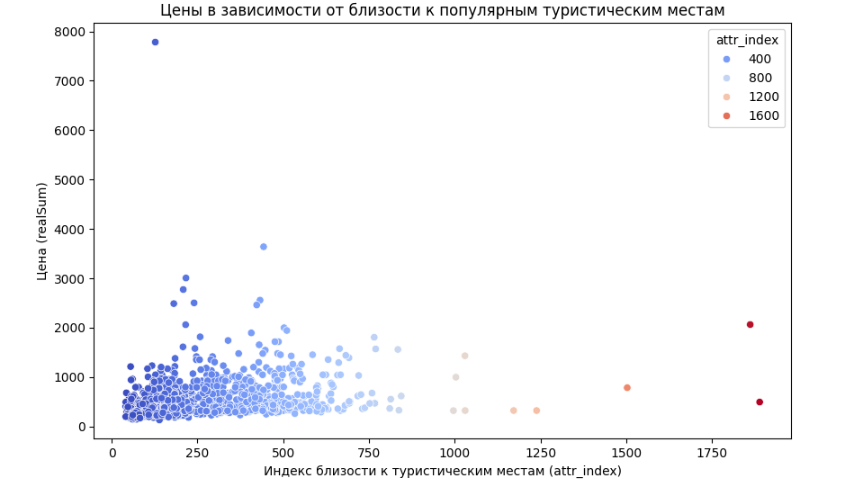
\includegraphics[width=1.0\textwidth]{fig-07}
		\caption{Листинги, расположенные ближе к популярным туристическим местам, имеют более высокие цены.}
	\end{figure}
	По диаграмме видим, что все точки сконцентрированны в основном у маленьких значений индекса, также имеется положительная корелляция 0.24, что говорит наличии положительный связи

	Рациональнее будет учесть, что чем меньше индекс близости тем больше цена, но если рассматривать большинство значений, котоый сконцентрированны от 0 до 750, то будем наблюдать положительный тренд(изходя из корреляционного анализа) и цена не будет зависеть от индекса.

\subsection{Цены в зависимости от района с высоким уровнем бизнеса}
\begin{python}
plt.figure(figsize=(10, 6))
sns.boxplot(data=df, x='biz', y='realSum')
plt.title('Prices depending on the area with a high level of business')
plt.xlabel('High level of business (biz)')
plt.ylabel('Price (realSum)')
plt.show()
\end{python}

	\begin{figure}[H]
		\centering
		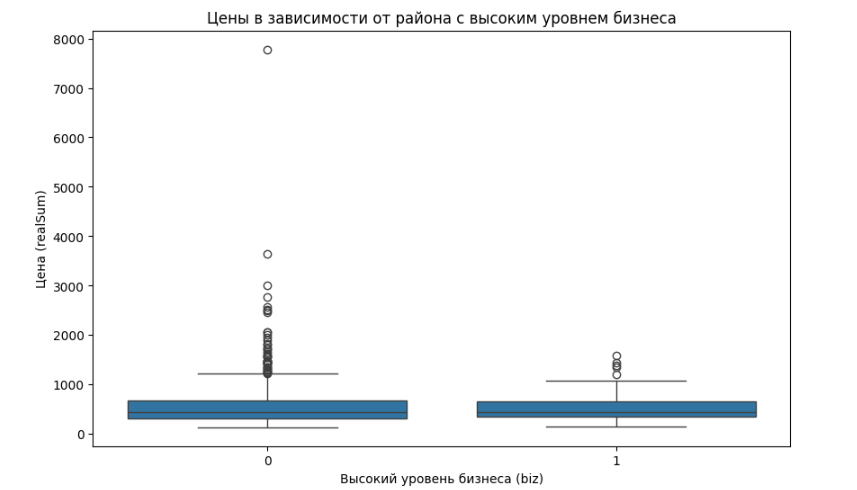
\includegraphics[width=1.0\textwidth]{fig-08}
		\caption{Листинги, находящиеся в районах с высоким уровнем бизнеса (biz), имеют более высокие цены.}
	\end{figure}
	По диаграмме с усами тяжело что-то сказать, но мы проводим т-тест, который показывает p-value 0.37, что говорит о том, что нет статистической разницы между переменными.

\subsection{Цены в зависимости от рейтинга чистоты}
\begin{python}
plt.figure(figsize=(10, 6))
sns.boxplot(data=df, x='cleanliness_rating', y='realSum')
plt.title('Prices depending on purity rating')
plt.xlabel('Purity rating (cleanliness_rating)')
plt.ylabel('Price (realSum)')
plt.show()

# t-test
median_cleanliness = df['cleanliness_rating'].median()
low_cleanliness_prices = df[df['cleanliness_rating'] < median_cleanliness]['realSum']
high_cleanliness_prices = df[df['cleanliness_rating'] >= median_cleanliness]['realSum']
t_stat_cleanliness, p_val_cleanliness = ttest_ind(low_cleanliness_prices, high_cleanliness_prices)
t_stat_cleanliness, p_val_cleanliness

\end{python}

	\begin{figure}[H]
		\centering
		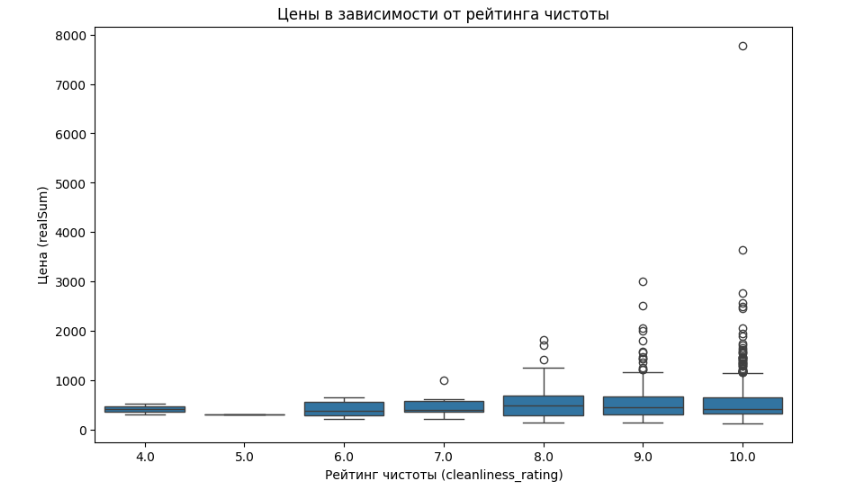
\includegraphics[width=1.0\textwidth]{fig-09}
		\caption{По диаграмме с усами видим, что значения примерно одинаковые, корреляция близка к 0, проведенный t-test показывает значение 0.8, что говорит нам об отстутствии статистической разницы средних.}
	\end{figure}
	По диаграмме с усами видим, что значения примерно одинаковые, корреляция близка к 0, проведенный t-test показывает значение 0.8, что говорит нам об отстутствии статистической разницы средних.

\subsection{Цены в зависимости от доступности для бронирования на несколько комнат}
\begin{python}
plt.figure(figsize=(10, 6))
sns.boxplot(data=df, x='multi', y='realSum')
plt.title('Prices depending on availability for booking multiple rooms')
plt.xlabel('Availability for booking multiple rooms (multi)')
plt.ylabel('Price (realSum)')
plt.show()

# t-test
mult_1 = df[df['multi'] == 0]['realSum']
mult_0 = df[df['multi'] == 1]['realSum']
t_stat_mult, p_val_mult = ttest_ind(mult_1, mult_0)
t_stat_mult, p_val_mult

# (3.502504162873662, 0.0004793932043132782)
\end{python}

	\begin{figure}[H]
		\centering
		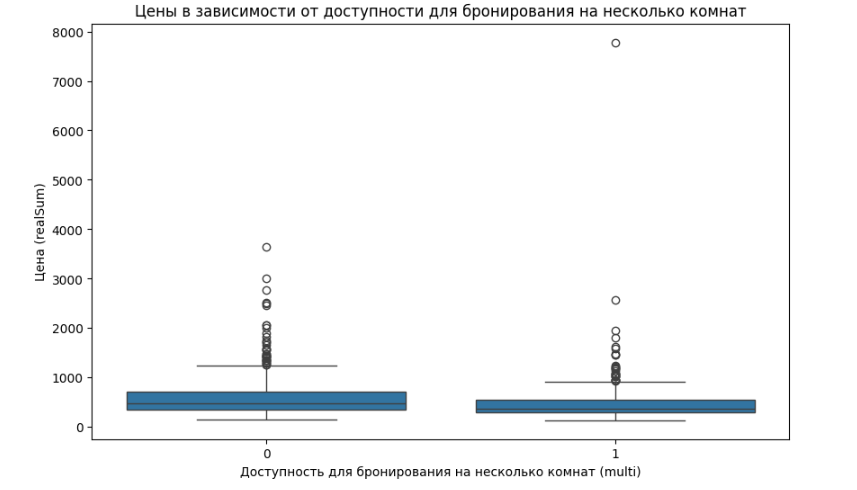
\includegraphics[width=1.0\textwidth]{fig-10}
		\caption{Листинги, доступные для бронирования на несколько комнат (multi), имеют более высокие ценe.}
	\end{figure}

\section{Выводы}
	На цену листинга в основном влияют следующие факторы:
	\begin{enumerate}
		\item Близость к центру города: Чем ближе листинг к центру, тем выше цена.

		\item Количество спален: Листинги с большим количеством спален имеют более высокие цены.

		\item Тип жилья: Целые дома или квартиры стоят дороже, чем отдельные комнаты.

		\item Доступность для бронирования на несколько комнат: Листинги, доступные для бронирования на несколько комнат, имеют более высокие цены.

		\item Рейтинг удовлетворенности гостей: чем больше рейтинг, тем дороже листинг.
	\end{enumerate}


\bibliographystyle{plain.bst}
\bibliography{reference}
\end{document}

